\documentclass[conference]{IEEEtran}
\IEEEoverridecommandlockouts
\usepackage{cite}
\usepackage{tabularx}
\usepackage{amsmath,amssymb,amsfonts}
\usepackage{graphicx}
\usepackage{textcomp}
\usepackage{xcolor}
\usepackage{url} % Added for better URL formatting
\usepackage{caption} % Added for subfigures if needed and figure notes
% \usepackage{amsmath}
\usepackage{algpseudocode}


\def\BibTeX{{\rm B\kern-.05em{\sc i\kern-.025em b}\kern-.08em
    T\kern-.1667em\lower.7ex\hbox{E}\kern-.125emX}}
\begin{document}

\title{\textbf{Analisis Penentuan Ketinggian Awal Air dalam Tangki Silinder Menggunakan Metode Numerik}}

\author{
\IEEEauthorblockN{Bonifasius Raditya Pandu Hendrianto}
\IEEEauthorblockA{\textit{Teknik Komputer} \\
\textit{Universitas Indonesia}\\
Depok, Indonesia \\
radityahendrianto@gmail.com}
}

\maketitle

\begin{abstract}
Penentuan parameter aliran fluida merupakan aspek krusial dalam berbagai aplikasi rekayasa. Studi ini berfokus pada penentuan ketinggian awal air ($H$) dalam sebuah tangki silinder yang mengalir melalui pipa panjang. Kecepatan air keluar ($v$) dari sistem ini dapat dihitung menggunakan persamaan yang melibatkan $H$, panjang pipa ($L$), waktu ($t$), dan percepatan gravitasi ($g$). Penelitian ini bertujuan untuk menerapkan dan membandingkan tiga metode numerik pencarian akar — metode grafis, \textit{bisecton method} (bisection), dan metode posisi palsu (false position) — untuk menentukan nilai $H$ yang memenuhi kondisi aliran tertentu. Hasil dari setiap metode akan dianalisis untuk mengevaluasi akurasi dan efisiensinya dalam menyelesaikan permasalahan ini, dengan kriteria penghentian $\epsilon_s = 1\%$.
\end{abstract}

\begin{IEEEkeywords}
KEYWORD: \\
ketinggian awal, aliran pipa, metode grafis, \textit{bisecton method}, metode posisi palsu, numerik, pencarian akar
\end{IEEEkeywords}

\section{PENDAHULUAN}

Dalam disiplin ilmu mekanika fluida, analisis aliran dari tangki penyimpanan melalui pipa merupakan salah satu problem fundamental dengan aplikasi yang luas, mulai dari sistem irigasi hingga proses industri. Salah satu parameter penting dalam analisis tersebut adalah ketinggian awal ($H_0$) fluida dalam tangki, karena parameter ini mempengaruhi kecepatan aliran keluar. Persamaan yang menggambarkan fenomena ini seringkali bersifat non-linear dan transenden, sehingga penyelesaian analitik untuk mencari parameter tertentu seperti ketinggian awal menjadi tidak praktis atau bahkan tidak mungkin dilakukan.

Tujuan utama dari penelitian ini adalah untuk mendemonstrasikan penerapan \textit{bisecton method} secara sistematis dalam menemukan solusi numerik untuk permasalahan aliran fluida yang diberikan. Untuk memfokuskan analisis, studi ini menggunakan serangkaian parameter yang telah ditetapkan: kecepatan target air adalah $v = 4 \, \text{m/s}$, panjang pipa $L = 5 \, \text{m}$, dan waktu $t = 3 \, \text{s}$. Implementasi \textit{bisecton method} akan dilakukan dengan menggunakan interval awal tebakan $[0, 2]$ meter dan kriteria penghentian berupa galat relatif perkiraan ($\epsilon_a$) yang lebih kecil dari $1\%$.

\section{DASAR TEORI}
Dinamika fluida adalah cabang dari mekanika fluida yang mempelajari bagaimana fluida (cairan dan gas) bergerak serta gaya yang bekerja padanya. Studi ini sangat penting dalam berbagai aplikasi rekayasa, mulai dari desain pesawat hingga sistem perpipaan. Prinsip fundamental yang mendasari dinamika fluida adalah hukum kekekalan massa, momentum, dan energi. Dari prinsip-prinsip ini, diturunkan persamaan-persamaan yang menggambarkan hubungan antara properti fluida seperti tekanan, kecepatan, dan ketinggian. Salah satu persamaan paling terkenal dalam dinamika fluida adalah Persamaan Bernoulli, yang menghubungkan energi kinetik, energi potensial, dan energi aliran fluida di sepanjang garis aliran. Persamaan ini menjadi dasar untuk memahami fenomena seperti gaya angkat pada sayap pesawat dan aliran air dalam pipa.

Salah satu aplikasi langsung dari Prinsip Bernoulli adalah Hukum Torricelli. Hukum ini, yang dirumuskan oleh Evangelista Torricelli, secara spesifik menjelaskan kecepatan aliran keluar (efluks) suatu fluida dari sebuah lubang kecil pada sebuah wadah atau tangki. Dalam kondisi ideal, di mana lubang dianggap kecil dibandingkan luas penampang tangki dan viskositas diabaikan, hukum ini menyatakan bahwa kecepatan aliran keluar, $v$, sama dengan kecepatan yang akan diperoleh sebuah benda jika jatuh bebas dari ketinggian $h$, yaitu ketinggian permukaan fluida di atas lubang. Secara matematis, hukum ini dinyatakan sebagai $v = \sqrt{2gh}$, dengan $g$ adalah percepatan gravitasi. Hukum ini memberikan fondasi teoretis yang kuat untuk menganalisis sistem aliran sederhana, seperti yang digambarkan pada studi kasus ini.

Namun, Hukum Torricelli merupakan model ideal. Dalam sistem nyata yang melibatkan pipa panjang, faktor-faktor seperti gesekan (friksi) dan efek transien (perubahan seiring waktu) saat fluida mulai bergerak menjadi signifikan. 

\begin{figure}[htbp]
  \centering
  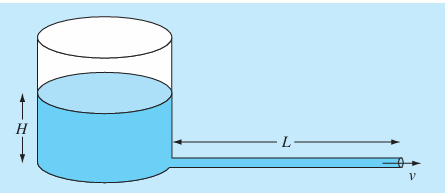
\includegraphics[width=\columnwidth]{src/5.15.png}
  \caption{Diagram skematik sistem tangki silinder dan pipa pembuangan.}
  \label{fig:sistem_tangki}
\end{figure}

\begin{equation}
v = \sqrt{2gH} \tanh\left(\frac{\sqrt{2gH}}{2L}t\right)
\label{eq:kecepatan_air}
\end{equation}
dimana:
\begin{itemize}
    \item $g$ adalah percepatan gravitasi ($9.81 \text{ m/s}^2$) 
    \item $H$ adalah ketinggian awal air dalam tangki (m) 
    \item $L$ adalah panjang pipa (m) 
    \item $t$ adalah waktu yang telah berlalu (s) 
\end{itemize}

Fungsi tangen hiperbolik ($\tanh$) dalam persamaan ini bertugas untuk merepresentasikan bagaimana kecepatan secara bertahap meningkat dari nol menuju kondisi tunaknya, dengan mempertimbangkan panjang pipa $L$ dan waktu $t$. Karena variabel ketinggian $H$ muncul di dalam dan di luar fungsi transendental ini, persamaan tersebut tidak dapat diselesaikan secara aljabar untuk mencari nilai $H$. Oleh karena itu, diperlukan pendekatan numerik untuk menemukan akarnya. Metode seperti \textit{bisecton method} (\textit{bisection}) dan posisi palsu (\textit{false position}) adalah teknik iteratif yang dapat digunakan untuk menghitung nilai $H$ dengan tingkat akurasi yang diinginkan, sesuai dengan parameter yang diberikan dalam masalah.

\section{DATA PENGUJIAN}
Terdapat beberapa variabel yang digunakan dalam perhitungan numerik \textit{bisection method ini}. Parameter waktu (t), panjang saluran (L), dan percepatan gravitasi akan berperan sebagai variabel kontrol karena nilainya sudah ditetapkan diawal. Parameter yang dijaga konstan selama simulasi adalah:
\begin{itemize}
    \item Percepatan gravitasi ($g$) sebesar $9.81 \, \text{m/s}^2$.
    \item Panjang saluran ($L$) sepanjang $5.00 \, \text{m}$.
    \item Waktu yang telah berlalu ($t$) selama $3.00 \, \text{s}$.
\end{itemize}

Parameter tinggi air ($H_0$) akan berperan sebagai variabel bebas dimana nilai ini akan divariasikan untuk mendapatkan hasil beragam sehingga nilai error akan semakin valid. Perhitungan numerik dimulai dengan nilai $H = 1.00 \, \text{m}$ dan ditingkatkan secara bertahap dengan skala interval $2.00 \, \text{m}$ untuk setiap uji coba berikutnya. Total uji coba perhitungan numerik adalah 10x sehingga tingg air ($H_0$) maksimal adalah $H = 19.00 \, \text{m}$. 

Hasil dari perhitungan numerik ini adalah kecepatan aliran air (v) sebagai variabel terikat. Rumus yang digunakan mengandung unsur prinsip bernoulli. Seluruh data hasil keluaran dari program simulasi ini dirangkum secara lengkap pada Tabel \ref{tab:data_simulasi}.

\begin{table}[htbp]
\centering
\caption{Data Uji Coba Kecepatan Aliran}
\label{tab:data_uji_rapi}
\renewcommand{\arraystretch}{1.2}
\begin{tabular}{|c|r|r|r|}
\hline
\textbf{Uji Coba} & \multicolumn{1}{c|}{\textbf{H (m)}} & \multicolumn{1}{c|}{\textbf{L (m)}} & \multicolumn{1}{c|}{\textbf{t (s)}} \\
\hline
1  & 5.00 & 5.00 & 3.00  \\
2  & 3.00 & 5.00 & 3.00  \\
3  & 5.00 & 5.00 & 3.00  \\
4  & 7.00 & 5.00 & 3.00  \\
5  & 9.00 & 5.00 & 3.00  \\
6  & 11.00 & 5.00 & 3.00 \\
7  & 13.00 & 5.00 & 3.00 \\
8  & 15.00 & 5.00 & 3.00 \\
9  & 17.00 & 5.00 & 3.00 \\
10 & 19.00 & 5.00 & 3.00 \\
\hline
\end{tabular}
\end{table}

\section{METODE PENYELESAIAN}

Metode yang dipakai untuk menyelesaikan permasalahan ini adalah \textbf{\textit{bisecton method} (bisection method)}. Metode ini merupakan metode pencarian akar yang didasarkan pada teorema nilai antara. Prosesnya dimulai dengan menentukan dua tebakan awal, $x_l$ (batas bawah) dan $x_u$ (batas atas), yang harus mengurung akar, yang berarti perkalian nilai fungsi pada kedua titik tersebut harus negatif ($f(x_l)f(x_u) < 0$). Estimasi akar berikutnya, $H_0$, dihitung sebagai titik tengah interval:
\begin{equation}
    H_0 = \frac{x_l + x_u}{2}
\end{equation}
Interval kemudian diperbarui untuk iterasi selanjutnya. Galat relatif perkiraan ($\epsilon_a$) dihitung untuk mengukur perubahan antara estimasi akar yang baru dan yang sebelumnya, menggunakan rumus:
\begin{equation}
    \epsilon_a = \left|\frac{x_{r}^{\text{baru}} - x_{r}^{\text{lama}}}{x_{r}^{\text{baru}}}\right| \times 100\%
\end{equation} 
Iterasi akan berhenti ketika nilai $\epsilon_a$ lebih kecil atau sama dengan kriteria penghentian yang ditentukan ($\epsilon_s$).

Berikut merupakan pseudocode untuk pengimplementasian \textit{bisection method}:
\begin{flushleft}
\begin{algorithmic}[1]
    \State Definisikan fungsi $f(H) \gets \sqrt{2gH} \tanh\left(\frac{\sqrt{2gH}}{2L}t\right) - v$.
    \State Inisialisasi parameter yang diperlukan: batas awal $x_l$ dan $x_u$, serta kriteria berhenti $\epsilon_s$.
    \State Inisialisasi variabel penyimpan: $H_0^{\text{lama}} \gets 0$.
    \While{true}
        \State Hitung estimasi akar baru: $H_0 \gets \frac{x_l + x_u}{2}$.
        \State Hitung galat relatif perkiraan: $\epsilon_a \gets \left| (H_0 - H_0^{\text{lama}}) / H_0 \right| \times 100\%$.
        \If{$\epsilon_a \le \epsilon_s$}
            \State \textbf{break}
        \EndIf
        \If{$f(x_l) \cdot f(H_0) < 0$}
            \State Perbarui batas atas: $x_u \gets H_0$.
        \Else
            \State Perbarui batas bawah: $x_l \gets H_0$.
        \EndIf
        \State Simpan estimasi saat ini untuk iterasi berikutnya: $H_0^{\text{lama}} \gets H_0$.
    \EndWhile
    \State \Return $H_0$
\end{algorithmic}
\end{flushleft}

\clearpage
\section{ANALISA HASIL EKSPERIMEN}
Berikut merupakan hasil kecepatan aliran air yang diperoleh dari prinsip bernoulli dengan ketinggian variatif interval 2m.
\begin{table}[htbp]
\centering
\caption{Hasil Simulasi Kecepatan Aliran Air}
\label{tab:simulasi_aliran_air}
\renewcommand{\arraystretch}{1.2} % Memberi sedikit ruang ekstra antar baris
\begin{tabular}{|c|r|r|r|r|}
\hline
\textbf{Uji Coba} & \textbf{H (m)} & \textbf{L (m)} & \textbf{t (s)} & \textbf{Kecepatan (m/s)} \\
\hline
1  & 1.00  & 5.00 & 3.00 & 3.849030  \\
2  & 3.00  & 5.00 & 3.00 & 7.519812  \\
3  & 5.00  & 5.00 & 3.00 & 9.852684  \\
4  & 7.00  & 5.00 & 3.00 & 11.698524 \\
5  & 9.00  & 5.00 & 3.00 & 13.279184 \\
6  & 11.00 & 5.00 & 3.00 & 14.686449 \\
7  & 13.00 & 5.00 & 3.00 & 15.968396 \\
8  & 15.00 & 5.00 & 3.00 & 17.154012 \\
9  & 17.00 & 5.00 & 3.00 & 18.262441 \\
10 & 19.00 & 5.00 & 3.00 & 19.307152 \\
\hline
\end{tabular}
\end{table}

Setelah mendapatkan data kecepatan aliran air dari berbagai ketinggian awal, langkah selanjutnya adalah mencari akar dari fungsi yang menghubungkan ketinggian awal ($H$) dengan kecepatan aliran ($v$) dengan menggunakan metode numerik \textit{bisection method}. Tabel \ref{tab:hasil_bisection} di bawah ini menunjukkan hasil iterasi dari metode bisection untuk mencari nilai ketinggian awal yang diperlukan untuk mencapai kecepatan aliran $v = 4 \, \text{m/s}$:
\begin{table}[htbp]
\centering
\caption{Hasil Iterasi \textit{bisection method} untuk Mencari H}
\label{tab:hasil_bisection}
\renewcommand{\arraystretch}{1.2}
\begin{tabular}{|c|c|c|c|r|c|}
\hline
\textbf{Iterasi} & $\boldsymbol{x_l}$ & $\boldsymbol{x_u}$ & $\boldsymbol{x_r}$ & \multicolumn{1}{c|}{$\boldsymbol{f(x_r)}$} & $\boldsymbol{\epsilon_a (\%)}$ \\
\hline
1 & 0.000000 & 2.000000 & 1.000000 & -0.15097 & - \\
2 & 1.000000 & 2.000000 & 1.500000 & 1.01452 & 33.33 \\
3 & 1.000000 & 1.500000 & 1.250000 & 0.46467 & 20.00 \\
4 & 1.000000 & 1.250000 & 1.125000 & 0.16543 & 11.11 \\
5 & 1.000000 & 1.125000 & 1.062500 & 0.00934 & 5.88  \\
6 & 1.000000 & 1.062500 & 1.031250 & -0.07026 & 3.03  \\
7 & 1.031250 & 1.062500 & 1.046875 & -0.03032 & 1.49  \\
8 & 1.046875 & 1.062500 & \textbf{1.054688} & -0.01046 & \textbf{0.74} \\
\hline
\end{tabular}
\end{table}

Nilai pada kolom ini didapatkan dengan memasukkan setiap nilai \textbf{$H_0$} (estimasi akar pada iterasi tertentu) ke dalam fungsi $f(H)$ yang ingin dicari akarnya. Iterasi ke-1 adalah nilai tengah dari interval 0 dan 2, yakni 1.0 sebagai nilai bagi dua.
Perhitungan untuk Iterasi ke-2:
\begin{enumerate}
    \item Identifikasi nilai $x_r$ yang relevan:
    \begin{itemize}
        \item $x_{r, \text{baru}}$ (dari iterasi ke-2) = \textbf{1.500000}
        \item $x_{r, \text{lama}}$ (dari iterasi ke-1) = \textbf{1.000000}
    \end{itemize}
    
    \item Masukkan ke dalam rumus:
    $\epsilon_a = \left| \frac{1.500000 - 1.000000}{1.500000} \right| \times 100\%$
    
    \item Selesaikan kalkulasi:
    $\epsilon_a = \left| \frac{0.5}{1.5} \right| \times 100\% = 0.3333... \times 100\% = \textbf{33.33\%}$
\end{enumerate}
Perhitungan untuk Iterasi ke-3:
\begin{enumerate}
    \item Identifikasi nilai $x_r$ yang relevan:
    \begin{itemize}
        \item $x_{r, \text{baru}}$ (dari iterasi ke-3) = \textbf{1.250000}
        \item $x_{r, \text{lama}}$ (dari iterasi ke-2) = \textbf{1.500000}
    \end{itemize}
    
    \item Masukkan ke dalam rumus:
    $\epsilon_a = \left| \frac{1.250000 - 1.500000}{1.250000} \right| \times 100\%$
    
    \item Selesaikan kalkulasi:
    $\epsilon_a = \left| \frac{-0.25}{1.25} \right| \times 100\% = 0.2 \times 100\% = \textbf{20.00\%}$
\end{enumerate}

Perhitungan selesai sampai nilai galat relatif mencapai nilai yang lebih kecil dari kriteria penghentian yang ditentukan (pada kasus ini, nilai $\epsilon_s = 1\%$). Pada kasus ini, iterasi terakhir adalah 8\\
Perhitungan untuk Iterasi ke-8:
\begin{enumerate}
    \item Identifikasi nilai $x_r$ yang relevan:
    \begin{itemize}
        \item $x_{r, \text{baru}}$ (dari iterasi ke-8) = \textbf{1.054688}
        \item $x_{r, \text{lama}}$ (dari iterasi ke-7) = \textbf{1.046875}
    \end{itemize}
    
    \item Masukkan ke dalam rumus:
    $\epsilon_a = \left| \frac{1.054688 - 1.046875}{1.054688} \right| \times 100\%$
    
    \item Selesaikan kalkulasi:
    $\epsilon_a = \left| \frac{0.007813}{1.054688} \right| \times 100\% = 0.00741... \times 100\% = \textbf{0.74\%}$
\end{enumerate}

Perhitungan dihentikan pada \textbf{iterasi ke-8} karena nilai galat relatif perkiraan ($\epsilon_a = 0.74\%$) telah lebih kecil dari kriteria penghentian yang ditentukan, yakni $1\%$. Dengan demikian, nilai ketinggian awal ($H$) yang diperlukan untuk mencapai kecepatan aliran $4 \, \text{m/s}$ adalah sekitar \textbf{1.054688 meter}.

\section{KESIMPULAN}

Penelitian ini bertujuan untuk menentukan ketinggian awal air ($H$) dalam sebuah tangki silinder yang diperlukan untuk menghasilkan kecepatan aliran keluar sebesar $4 \, \text{m/s}$ melalui pipa panjang. Karena sifat transendental dari persamaan aliran yang digunakan, solusi analitik tidak dapat dicapai, sehingga metode numerik pencarian akar, khususnya \textit{bisecton method} (\textit{bisection method}), diterapkan untuk menyelesaikan masalah ini. Berdasarkan hasil perhitungan iteratif dengan kriteria penghentian galat relatif di bawah $1\%$, ditemukan bahwa nilai ketinggian awal yang dibutuhkan adalah sekitar \textbf{1.054688 meter}. Hasil ini diperoleh setelah 8 kali iterasi, di mana galat relatif perkiraan ($\epsilon_a$) telah mencapai $0.74\%$. Studi kasus ini berhasil menunjukkan bahwa \textit{bisecton method} merupakan pendekatan yang andal dan konvergen untuk menyelesaikan permasalahan rekayasa non-linear yang kompleks, serta memberikan hasil yang akurat untuk perancangan sistem fluida.

\section{LINK GITHUB}
Berikut adalah link GitHub dari kelompok kami (jika ada implementasi kode):
\url{https://github.com/BonifasiusRaditya/TugasPemogramanB} % Placeholder

\begin{thebibliography}{00}
\bibitem{ref1} F. M. White, \textit{Fluid Mechanics}, 8th ed. New York: McGraw-Hill Education, 2016.
\bibitem{ref2} S. C. Chapra and R. P. Canale, \textit{Numerical Methods for Engineers}, 7th ed. New York: McGraw-Hill Education, 2015.
\bibitem{ref3} F. M. White, \textit{Fluid Mechanics}, 8th ed. New York: McGraw-Hill Education, 2016.
\end{thebibliography}
% Referensi lain yang relevan dapat ditambahkan di sini,
% misalnya buku teks mengenai metode numerik atau mekanika fluida.
\vspace{12pt}
% \color{red}
% IEEE conference templates contain guidance text for composing and formatting conference papers. Please ensure that all template text is removed from your conference paper prior to submission to the conference. Failure to remove the template text from your paper may result in your paper not being published.

\section{ANALISA HASIL EKSPERIMEN}

Analisis ini berfokus pada penyelesaian numerik untuk menemukan nilai ketinggian awal ($H$) yang akan menghasilkan kecepatan aliran target $v=4 \, \text{m/s}$. Metode yang digunakan adalah \textit{bisection method} dengan parameter awal sebagai berikut:
\begin{itemize}
    \item Fungsi target: $f(H) = \sqrt{2gH} \tanh\left(\frac{\sqrt{2gH}}{2L}t\right) - 4 = 0$
    \item Interval awal: $[x_l, x_u] = [0, 2]$
    \item Kriteria berhenti: $\epsilon_s = 1\%$
\end{itemize}

Proses pencarian akar dilakukan secara iteratif. Setiap iterasi menghasilkan estimasi akar baru ($x_r$) dan galat relatif perkiraan ($\epsilon_a$) yang dibandingkan dengan kriteria berhenti. Seluruh langkah perhitungan iteratif hingga solusi ditemukan dirangkum pada Tabel \ref{tab:hasil_bisection}.

\subsection*{Kesimpulan Hasil}
Perhitungan dihentikan pada \textbf{iterasi ke-8} karena nilai galat relatif perkiraan ($\epsilon_a = 0.74\%$) telah lebih kecil dari kriteria penghentian yang ditentukan ($\epsilon_s = 1\%$). Dengan demikian, nilai ketinggian awal ($H$) yang diperlukan untuk mencapai kecepatan aliran $4 \, \text{m/s}$ adalah sekitar \textbf{1.054688 meter}.

\end{document}